\section{Introduction}
This project explores predicting used car prices in Egypt using supervised machine learning~\citep{project-repository}. Having a clear, accurate price estimate helps buyers, sellers, and online platforms navigate the market with reliable, data-backed vehicle valuations. Because advertised car prices are continuous values measured in Egyptian pounds (EGP), we treat this task as a regression problem.

The dataset was built by scraping listings directly from Hatla2ee. After initial cleaning, the snapshot contains 14,556 used car listings, capturing key details such as model year, mileage, transmission type, fuel type, brand, model, and location. The advertised price serves as the target variable. While listing IDs and digital fingerprints are retained for validation and traceability, they are excluded as predictive features.

To customize the dataset for this study, I drew an 80\% simple random sample without replacement, using my TKH Student ID (2300632) as a fixed random seed. This created a reproducible working set of 11,645 listings. Following data preparation, this tailored dataset forms the foundation for training, comparing, and evaluating our regression models.

\section{Data Preparation}
Before drawing the working sample, I ran an initial exploratory data analysis (EDA) on the full 14,556-listing snapshot. This provided a detailed look at the dataset's overall characteristics and highlighted raw data quality issues. The analysis examined data types, missing values, feature cardinality, duplicate records, numerical distributions, category frequencies, and how potential predictors correlate with price.
The raw dataset contained no exact duplicate rows, listing IDs, or fingerprints. However, three features, ad\_date, color, and class, suffered from missing values and lacked predictive value, so they were removed. Visualizations and summary statistics showed that prices were heavily right-skewed, while year, mileage, brand, model, fuel type, transmission, and location stood out as strong potential predictors. Text-based mileage values, such as “30,000 KM,” were parsed and converted into a clean numerical column named mileage\_km.

See Figure~\ref{fig:numerical-distributions}.

\begin{figure}[H]
\centering
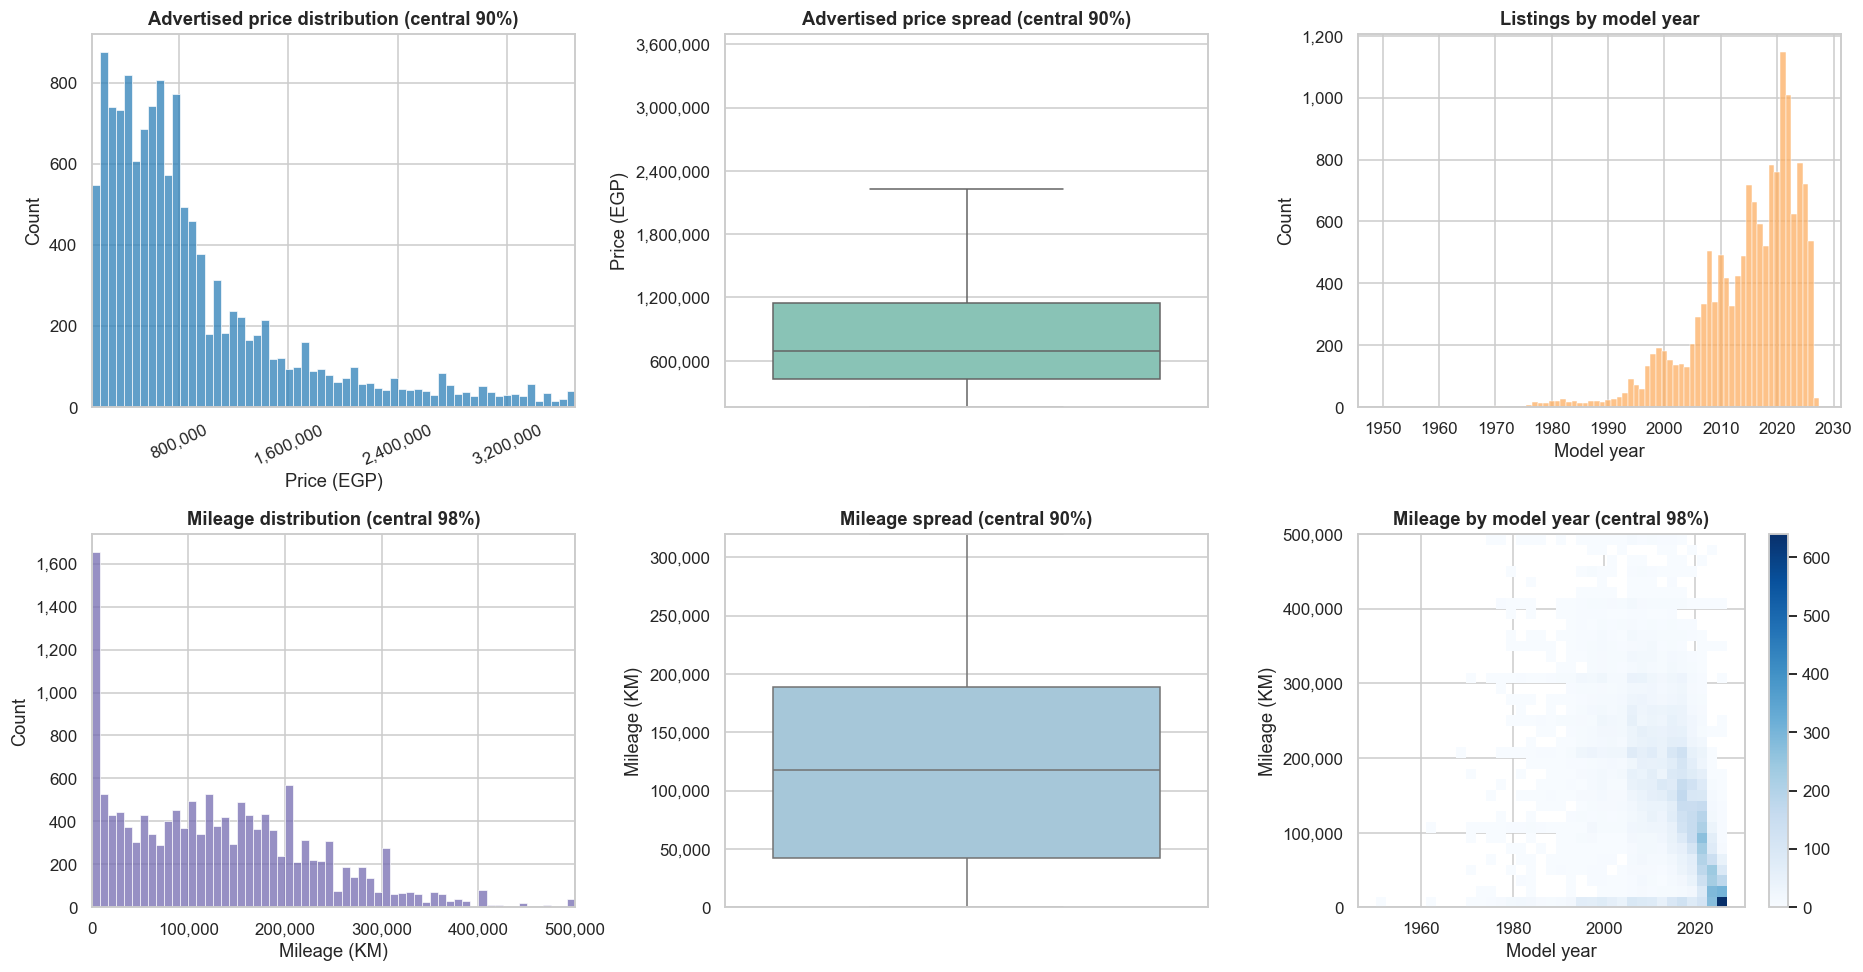
\includegraphics[width=\linewidth]{numerical_distributions.png}
\caption{Numerical distributions of price, model year, and mileage.}
\label{fig:numerical-distributions}
\end{figure}

Once the initial EDA was complete, I generated the personalized dataset by sampling 80\% of the cleaned listings without replacement using Student ID 2300632 as the seed. The resulting working set contains 11,645 listings. Because the sampling method is deterministic, re-running the process with the same seed will reproduce this exact working set.

Next, I applied strict data validation rules to the working sample. I filtered out listings missing mileage or reporting extreme values of 1,000,000 km or higher, as well as model years outside a realistic 1950–2026 range. Prices were required to be positive and below 100,000,000 EGP (all sampled listings met this price condition). In total, 33 records failed the mileage check and 23 failed the year check; accounting for overlap, 56 records were removed, leaving 11,589 listings for modeling.

Categorical features were standardized before modeling. Fuel entries were mapped into consistent categories, transmission types were grouped into Automatic, Manual, or Unknown, and cities were mapped to their broader governorates. Unmapped locations were retained as “Other / Unmapped” rather than removed. Finally, the title text was dropped because it redundantly repeated brand, model, and year info, while id and fingerprint were excluded from modeling as they represent unique listing identifiers rather than vehicle characteristics.

To prevent data leakage, transformations like imputation, scaling, and encoding are fitted strictly after splitting the data into training and test sets. Numerical features undergo median imputation followed by standardization, while categorical features use most-frequent-value imputation and one-hot encoding. This workflow ensures that test set information never influences the transformations learned during training.

\clearpage
\begin{thebibliography}{9}
\phantomsection
\addcontentsline{toc}{section}{References}
\bibitem{project-repository}
GitHub link: \url{https://github.com/yassienE4/MachineLearningCW}
\end{thebibliography}
